\section{Evaluation}
\label{sec:experiment}
In this section, we compare the optimized SGEMM performance in Gflop/s with NVIDIA CUBLAS. The $17\sim 25\%$ improvement confirms that the microarchitectural optimization makes sense when tuning SGEMM on GPUs. We further present a quantitative analysis of the effect of each individual optimization strategy and an estimation of the upper bound performance.

The experiments are conducted on NVIDIA K20m GPU, and the hardware configuration is summarized in Table~\ref{table:k20}. The compared CUBLAS is from CUDA $7.0$ version. In our experiments the sizes of matrix vary in $768\times768$, $1536\times1536$,$3072\times3072$,$6144\times6144$,$12288\times12288$.

\begin{table}[!t]
\caption{The configuration of NVIDIA Tesla K20m GPU.}
\centering
\scalebox{1.0} {
\begin{tabular}{|c|c|}
\hline
Metric& Value\\
\hline
SPs/SM &192\\
\hline
    SMs&13\\
\hline
Cores &2496\\
\hline
Frequency(MHz)&705\\
\hline
Memory Bus Width&320\\
\hline
Memory frequency&2600 Mhz\\
\hline
Bandwidth(GB/s)&208.0\\
\hline
Single FLOPS&3520\\
\hline
warp schedular per SM&4\\
\hline
dispatch unit/SM&8\\
\hline
Max registers/thread&256 \\
\hline
32-bit registers/SM&64K\\
\hline
LD/ST unit&32 \\
\hline
shared memory&48KB\\
\hline
L1 cache&16KB or 48KB\\
\hline
    L2 cache&1536KB\\
\hline
\end{tabular}
}
\label{table:k20}
\end{table}


\subsection{Overall Performance}
Figure~\ref{fig:sgemm_tn} reports the performance comparison of CUBLAS SGEMM and our optimized SGEMM.
Our SGEMM achieves $3104$ Gflop/s which efficiency is $3104/3520=88\%$. With the same matrix size, CUBLAS has $2509$ Gflop/s which efficiency is $71\%$. The comparison shows that our implementation achives $17\%$ performance improvement over CUBLAS.

As the figure shows, the overall trend is that performance increases with size of matrices. On one hand, the larger matrix size leads to a higher ratio of floating-point operations to matrix $C$ store operations, which is more close to the hardware arithmetic intensity. On the other hand, the larger matrix size increases workload of the threading CUDA cores, resulting in load balance. The numbers of block ranges from $[768/192,768/192]=[4,4]$ to $[12288/192, 12288/192]$ $=[64,64]$. Since Kepler has $13$ SMs in total, matrix of size $768\times 768$ suffers from load balance. Therefore, we observe that there is significant growth in Gflop/s from $768$ to $1536$ for both ours and CUBLAS. With respect to the ratio of performance improvement, the optimization has less effect on the smaller matrix size than the larger one. The reason is that the performance is increasingly bounded by the microarchitecture rather than memory due to the higher arithmetic intensity. Thus, our microarchitecture-level optimization plays more important role on tuning performance.

\begin{figure}[htbp]
\begin{center}
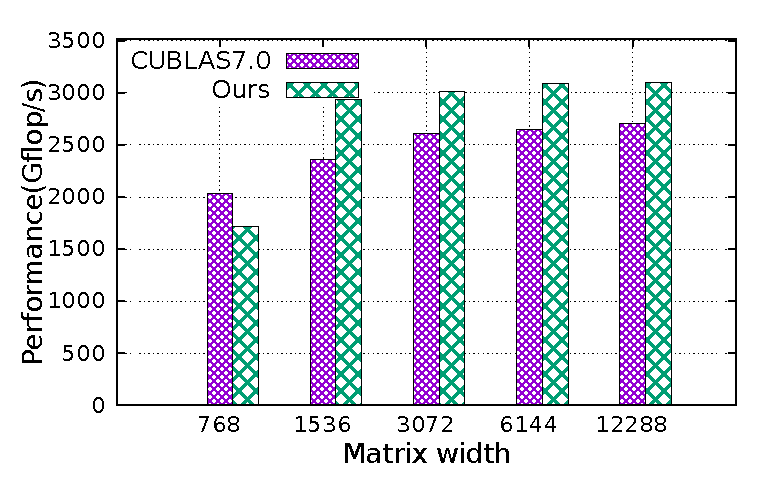
\includegraphics[scale=0.6]{sgemm_tn}
\caption{Performance comparison of CUBLAS and the optimized SGEMM }
\label{fig:sgemm_tn}
\end{center}
\end{figure}

\subsection{Performance Analysis}

\subsubsection{Register Blocking Size Influence}
Section~\ref{sec:background} summarized computation volumn and data movement volumn of blocking SGEMM algorithm.
The volumn of data moving from shared memory to global memory is $rx\times bk+ ry\times bk$, and computation volumn is $rx\times ry\times bk$. Thus, the computation and shared memory access ratio can be formulated as $\frac {rx\times ry\times bk} {rx\times bk+ ry\times bk} = \frac{1}{\frac{1}{rx} + \frac{1}{ry}}$.
This function implies that the larger register blocking, the higher computation shared memory ratio, and the optimal solution should be in the case of $rx=ry$. 
For global memory, it is the same conclusion.

However, Register blocking size is limited by number of registers per thread. 
%the maximum number of threads in one block.
In order to hide latency of shared memory, software pipelining using double
buffers is an efficient way. Each thread needs $rx\times ry$ registers to store result of $C$ submatrix, $rx$ and $ry$ to store a column of $A$
submatrix and a row of $B$ submatrix in current loop. In addition, the extra $rx$ and $ry$ registers are used for prefetching $A$ and $B$ from shared memory to
registers for next loop. Since the total number of registers should be less than $256$ on Kepler, we have the following equations:
\begin{equation}
    rx\times ry + rx\times 2 + ry\times 2 < 256
\label{f_register}
\end{equation}
Because the maximal number of register per thread is $256$ and data load must be aligned with $128$-bits when using {\tt LDG.128}, the blocking size might be $4\times 4$, $8\times 8$ and $12\times 12$. In fact, the blocking factor of $4\times 4$ leads to low data reuse in register files. Figure~\ref{fig:block} demonstrates $8\times8$ blocking and $12\times12$ blocking. $12\times12$ is better than
$8\times8$ in that, it has high computation memory ratio and higher instruction level parallelism. With respect to instruction scheduling optimization, $12\times12$ blocking has more slots to insert other {\tt non-FFMA} instructions, leaving more
space to schedule instructions, the overhead of {\tt LDS} can be amortized. Thus, the number of registers is $12*12+4*12=192$ used by both {\tt LD} and {\tt FFMA}, totally resulting $236$ registers with other address indices.The $65536$ registers per SM restricts us to launch $256$ threads at most. In our implementation, we have $256$ threads in a block. Each block of threads computes a $192\times 192$ submatrix of $C$ by multiply $A_{192,4}$ and $B_{4, 192}$, in which $4$ is the unroll factor.

\begin{figure}[htbp]
\begin{center}
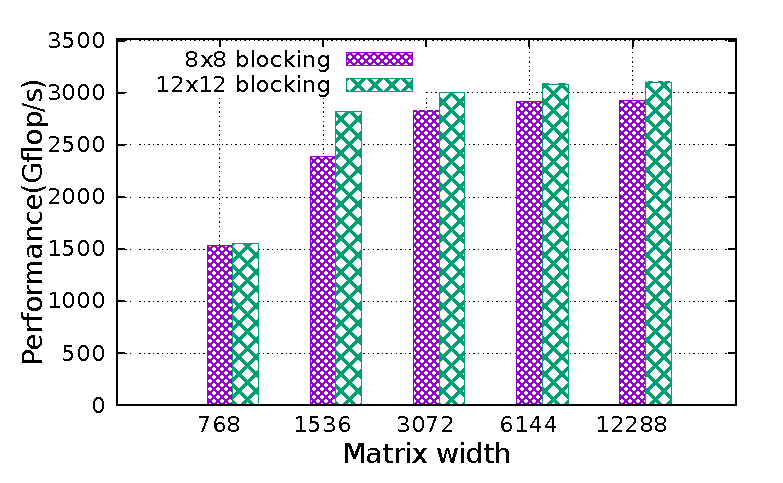
\includegraphics[scale=0.6]{block}
    \caption{Evaluation of different blocking size}
\label{fig:block}
\end{center}
\end{figure}
the active block per SM is one, occupancy is $256/1024=12.5\%$.
The occupancy is low which means the thread parallism is low, but our instruction level parallism is high. The high performance of SGEMM with low occupancy confirms that instruction level parallelism plays an important role on GPU~\cite{volkov2010better}.

\subsubsection{Profiling Microarchitectural Optimization}
In order to examine performance gain of different optimization strategies, we construct several intermediate implementations by incrementally applying the microarchitectural optimizations.

{\it Baseline:}~~The baseline involves conventional optimizations including register blocking, global
memory double buffering, shared memory double buffering and unrolling, rather than assembly level optimization.
For example, baseline use default $32-bit$ {\tt LD} rather than $128-bit$ {\tt LDG} to load data from global memory.
Register allocation for $C$ is allocated orderly from $0$ to $143$, then $A$ and $B$ matrices. In this case, {\tt
FFMA}s will have $368/(144*4)=63.89\%$ and $64/(144*4)=11.11\%$ 3-way bank conflicts. Baseline does not apply dual
issue optimization either.

{\it +Reg:}~~The register allocation pattern described in section~\ref{sec:assembler} is applied to eliminate register bank conflict. No
instruction scheduling change between this version and baseline version.

{\it +LD128:}~~Use wider global load instruction.
Kepler has an L1 data cache, but it is designed for local rather than global memory access. So {\tt LD} will not be L1-cached, it can be L2-cached.

{\it +LDG128:}~~Use the texture cached {\tt LDG} which is faster to replace L2-cached {\tt LD}. When {\tt LDG} is used, a {\tt TEXDEPBAR}~\cite{lukyanov2014efficient} is needed before using the data due to weak consistence of texture cache.

{\it +Dual:}~~Single issue is controlled by setting control code to $0x00$. Dual issue is fully enabled by utilizing the
pattern described in section~\ref{sec:assembler}. For dual issue version, {\tt NOP} may be inserted for instruction alignment.

\begin{figure}[htbp]
\begin{center}
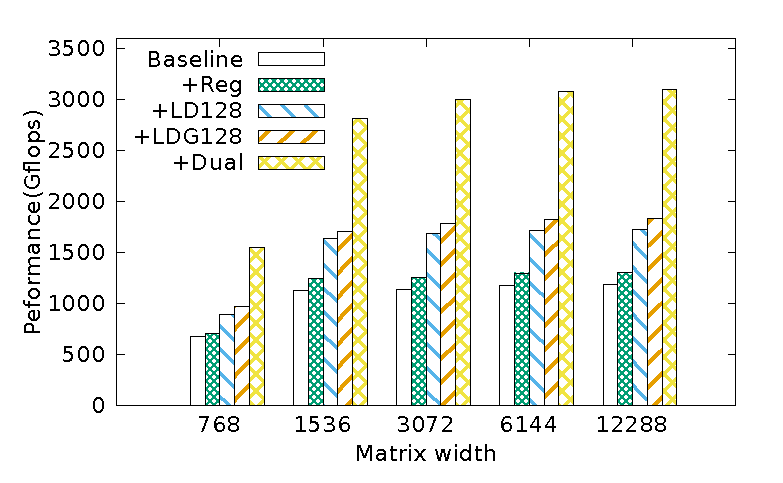
\includegraphics[scale=0.65]{tn_prof}
    \caption{Evaluation of the incremental optimizations.}
\label{fig:th_prof}
\end{center}
\end{figure}

Figure~\ref{fig:th_prof} illustrates performance gain of each optimization method.
As long as number of instructions is changed, instruction order needs rescheduling to achieve high performance.
Compared with the baseline implementation, $2.6X$ speedups are gained by applying all the optimization.
Register bank conflict eliminating improves around $10\%$. Wider load instruction improves $27\%\sim35\%$, texture cached
load instruction {\tt LDG} improves $5\%\sim12\%$. Dual issue improves the most, $84\%\sim106\%$.

\subsubsection{Upper Bound Analysis}

\jled{Add a Roofline figure?}

We estimate the upper bound factors: {\tt LDS}, {\tt LDG} and {\tt FFMA}. They correspond to $3$ kinds of resources, shared
memory, global memory and computation power. In register blocking loop, each thread compute $bm*bn*bk$, read $bm*bk$
and $bn*bk$ words. The upper bound of global memory bandwidth can be modeled as:
\begin{displaymath}
    \frac{2*bm*bn*bk}{4*(bm*bk + bn*bk)} = \frac{Gflop/s}{bandwidth}
\end{displaymath}
According to parameters in our SGEMM implementation, $bm=bn=192$, $bk=4$, $Gflop/s=3520$, so $73$ GB/s is the minimal
requirement for global memory bandwidth in order to achieve peak $3520$ Gflops.
For shared memory, inside each loop, $(rx*bk + ry * bk)*tx*ty$ words will be read from shared memory, in which $tx$,
$ty$ is block dimension, $rx$, $ry$ is register blocking size. The computation is $bm*bn*bk$. Based on computation
shared memory ration,
\begin{displaymath}
    \frac{2*bm*bk*bn}{4*tx*ty*(rx*bk + ry *bk)}  = \frac{Gflop/s}{bandwidth}
\end{displaymath}

On Kepler GPU the minimum bandwidth requirement is $1173$GB/s, and for each SM of Kepler, bandwidth requirement is
$1173/13=90$ GB/s.
The hardware can provide $200$GB/s global memory bandwidth and $2349$GB/s shared memory bandwidth, which is
higher than requirement, and hence neither bandwidth of shared width nor global memory will be bottleneck.

The loss to peak performance can be explained as the following reasons. As we have shown in Section~\ref{sec:assembler}, {\tt FFMA} throughput can achieve $97.67\%$. The loss is about $2.33\%$, which may comes from overhead of warp scheduler in {\tt FFMA} dual issue mode. The double-buffering algorithm can amortize the latency of {\tt LDS}.
With $12x12$ register blocking and $4$ times unrolling, there will be $144*4=576$ {\tt FFMA} instructions in the loop.
With our designed {\tt FFMA} dual issue pattern, every $6$ {\tt FFMA} needs $4$ clock cycles in the pipeline.
It needs $4*144*4/6=384$ clock cycles for each thread,  two $128$ bits {\tt LDG} instruction are needed.
We observe each {\tt LDG} has $10$ clock penalty, the total {\tt LDG} will cause $2*10/384 = 5.2\%$ loss. Other penalty comes from synchronization and writing $C$ matrix in the block.
